\section{Конструкторская часть}	
	\subsection{Use-Case диаграмма}
	На рисунках \ref{fig2:image}-\ref{fig4:image} приведены диаграммы вариантов использования для каждого актора, полная схема находится в приложении.
	
	\begin{figure}[ph!]
		\centering
		\begin{center}
			{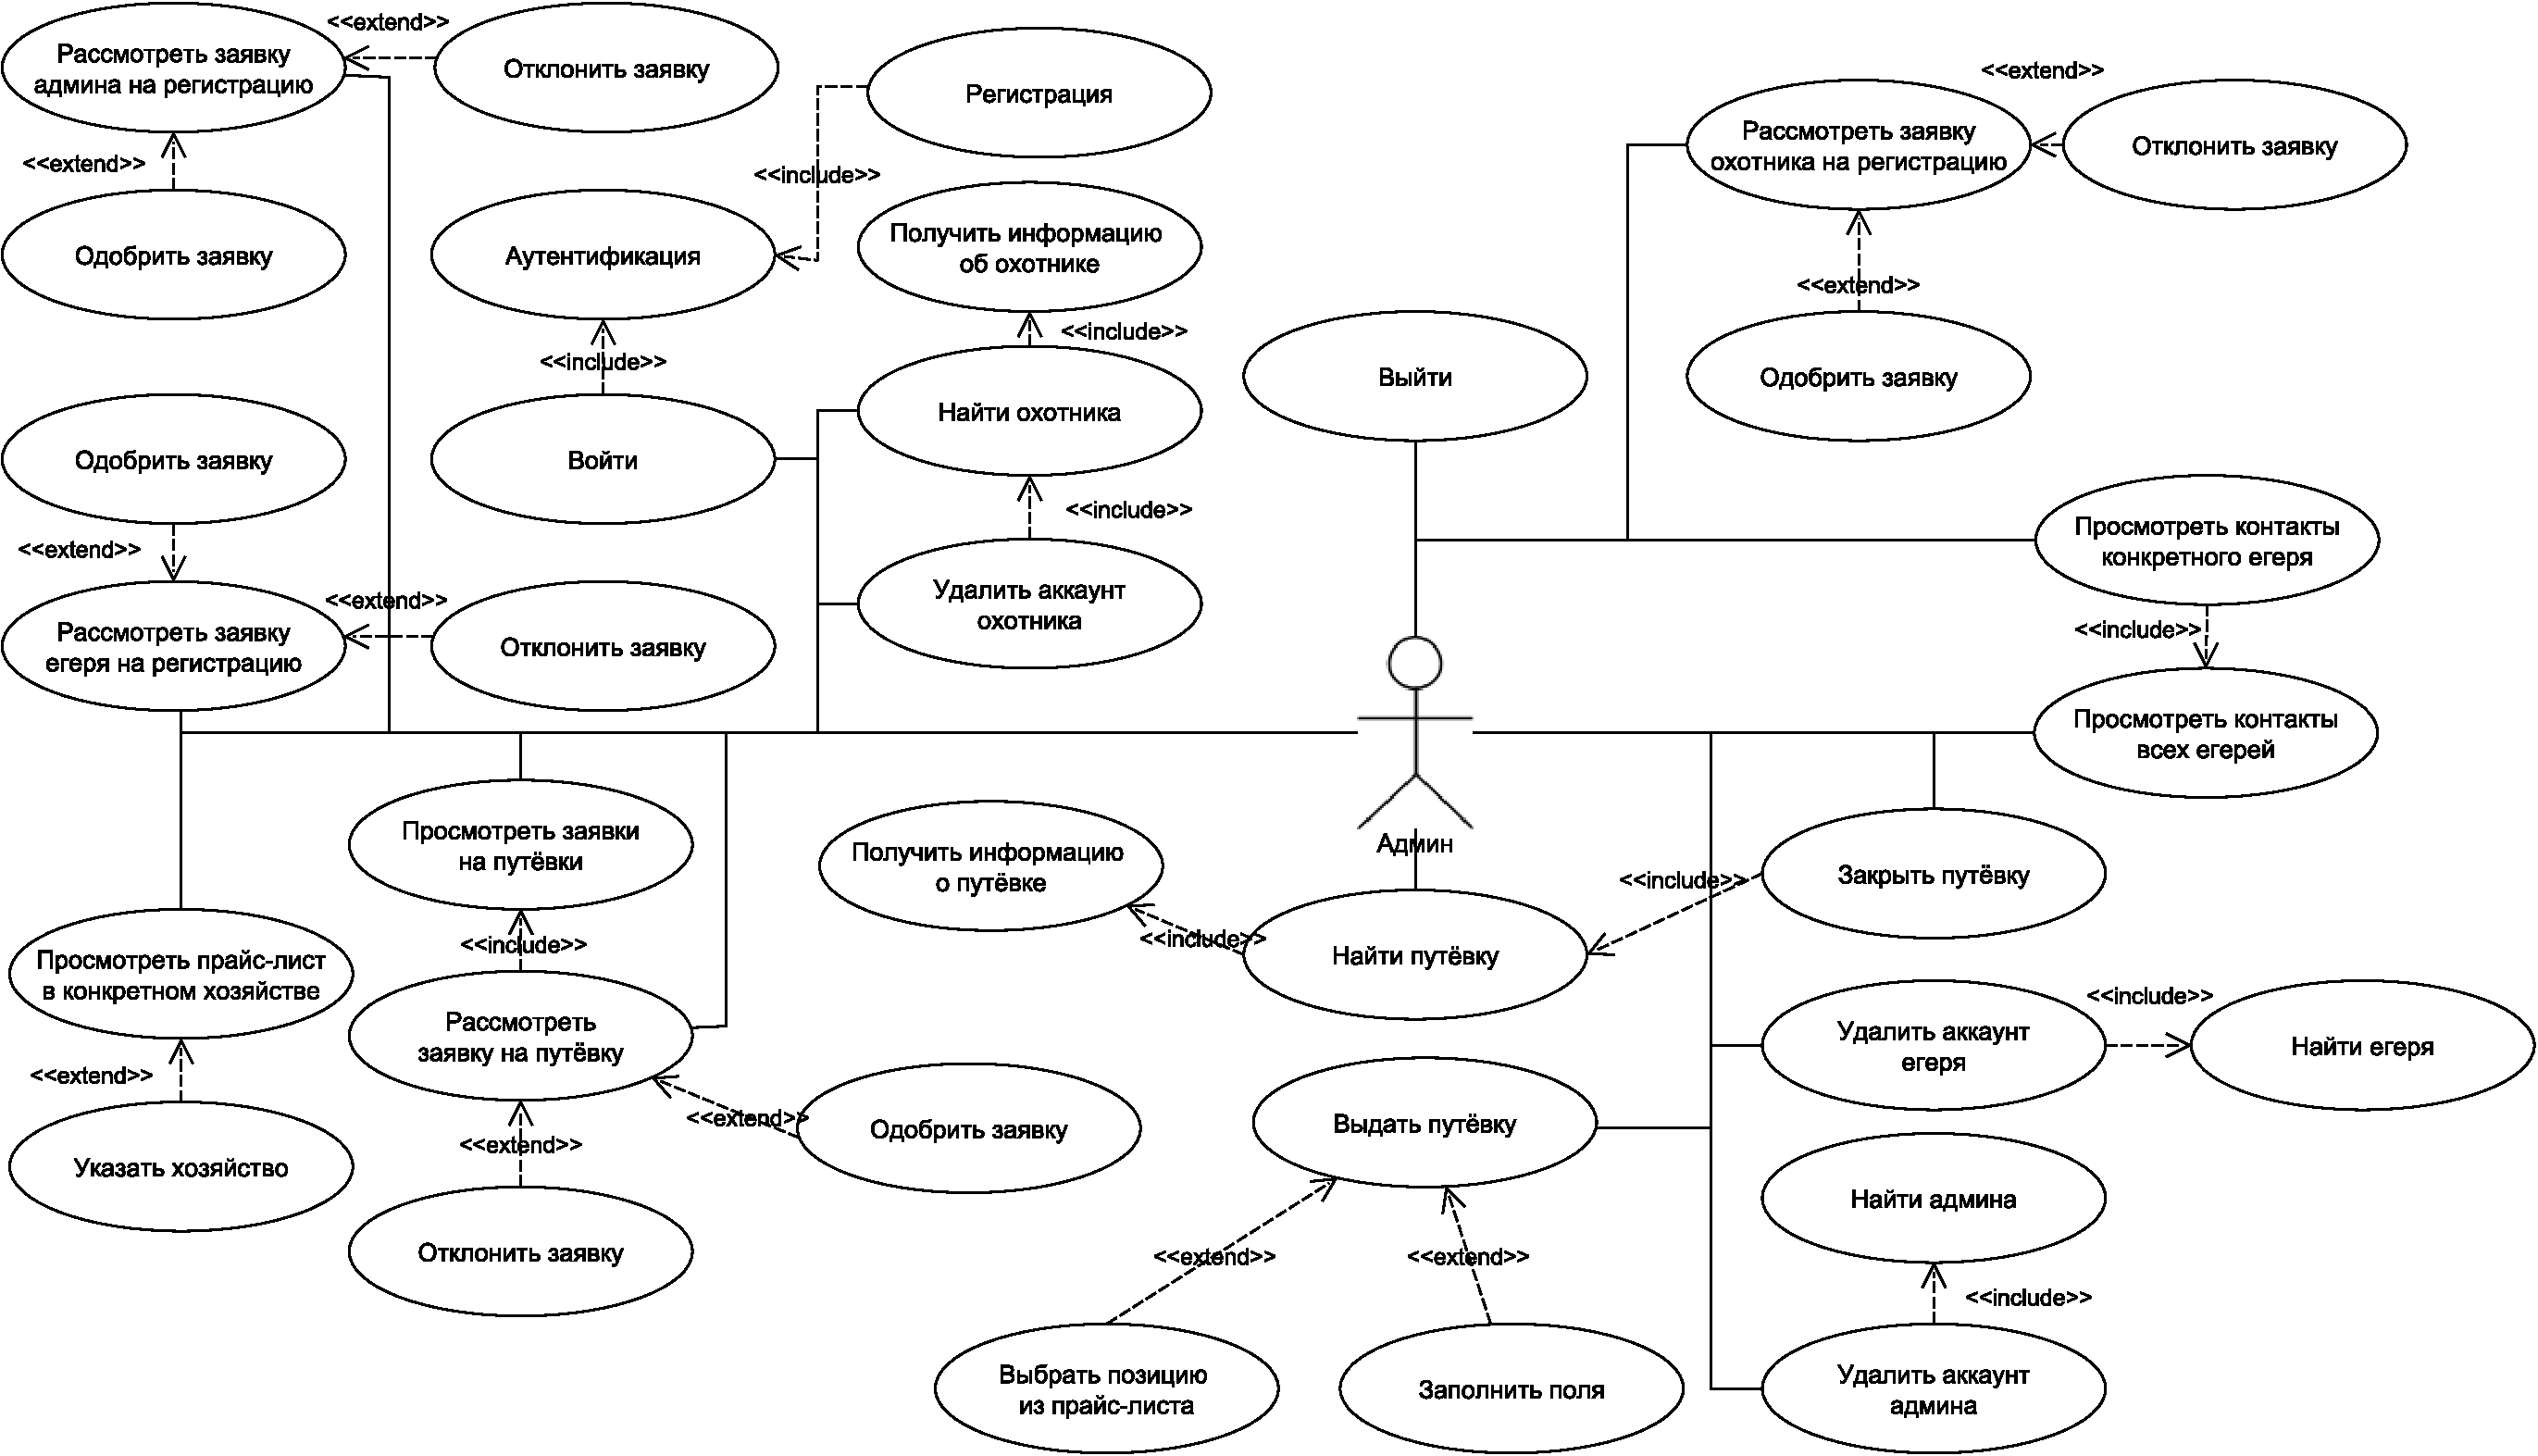
\includegraphics[scale=0.44, angle=90]{schemes/use-case_admin.pdf}}
			\caption{ER-диаграмма сущностей (администратор)}
			\label{fig2:image}
		\end{center}
	\end{figure}

	\begin{figure}[ph!]
		\centering
		\begin{center}
			{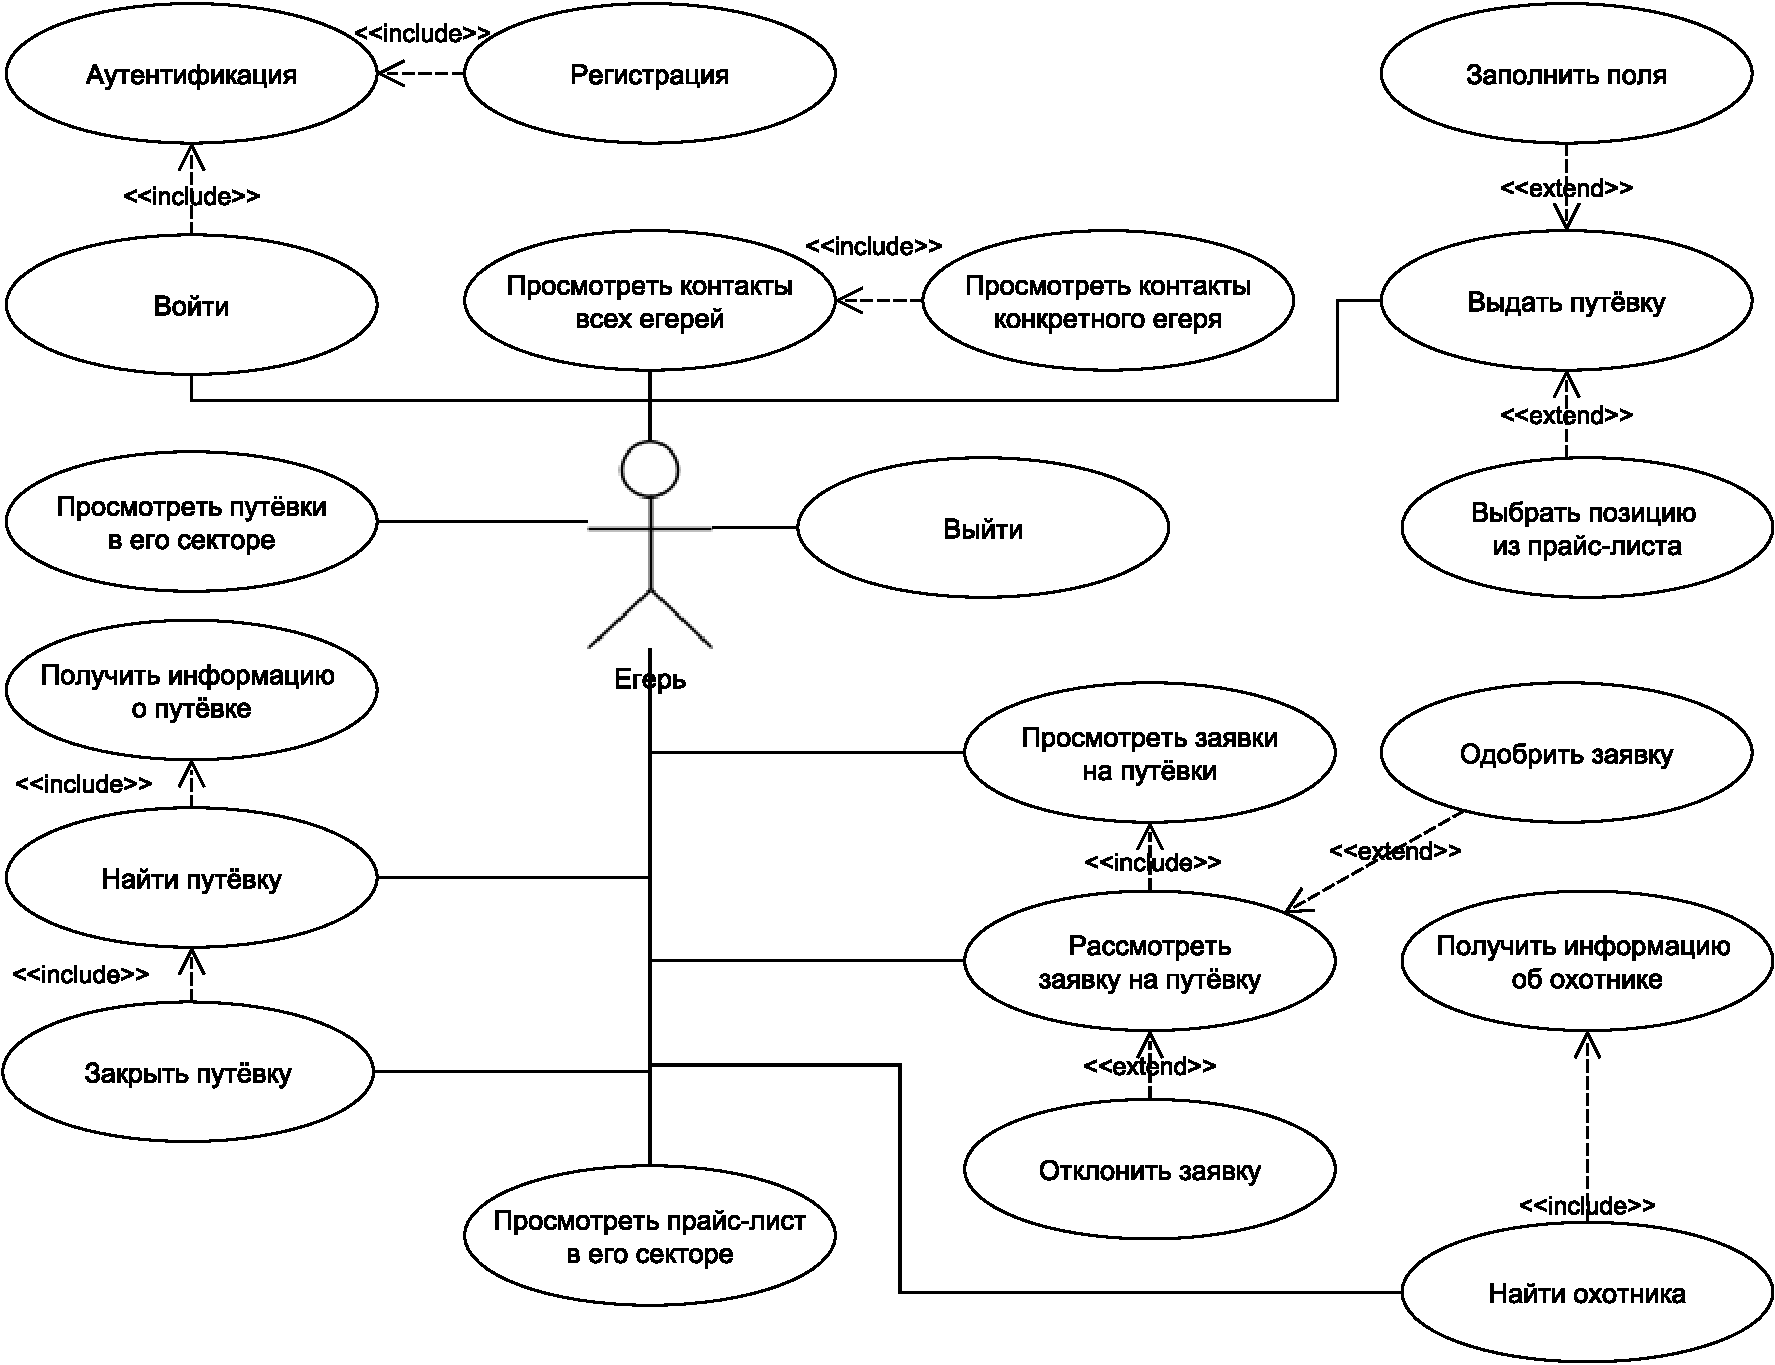
\includegraphics[scale=0.45]{schemes/use-case_huntsman.pdf}}
			\caption{ER-диаграмма сущностей (егерь)}
			\label{fig3:image}
		\end{center}
	\end{figure}

	\begin{figure}[ph!]
		\centering
		\begin{center}
			{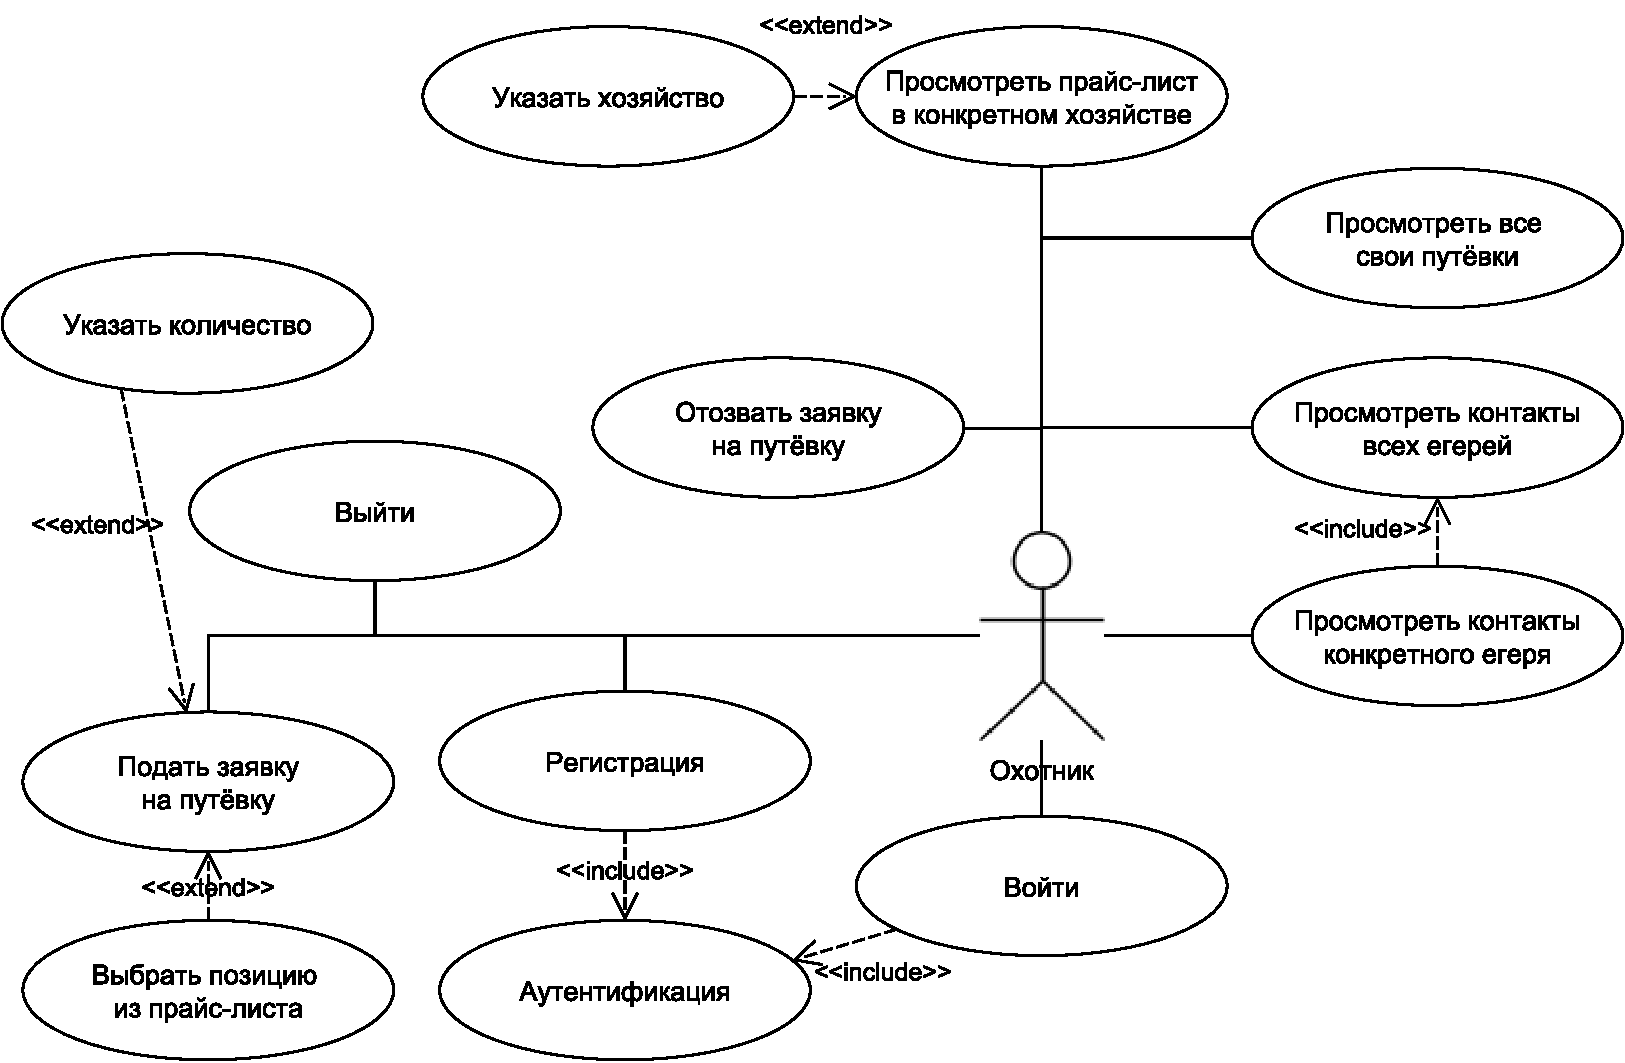
\includegraphics[scale=0.45]{schemes/use-case_hunter.pdf}}
			\caption{ER-диаграмма сущностей (охотник)}
			\label{fig4:image}
		\end{center}
	\end{figure}
	
	\newpage
	
	\subsection{ER-диаграмма сущностей БД}
	На рисунке \ref{fig5:image} приведена ER-диаграмма базы данных, на которой также указываются связи, поля таблиц и ключи.
	
	\begin{figure}[ph!]
		\centering
		\begin{center}
			{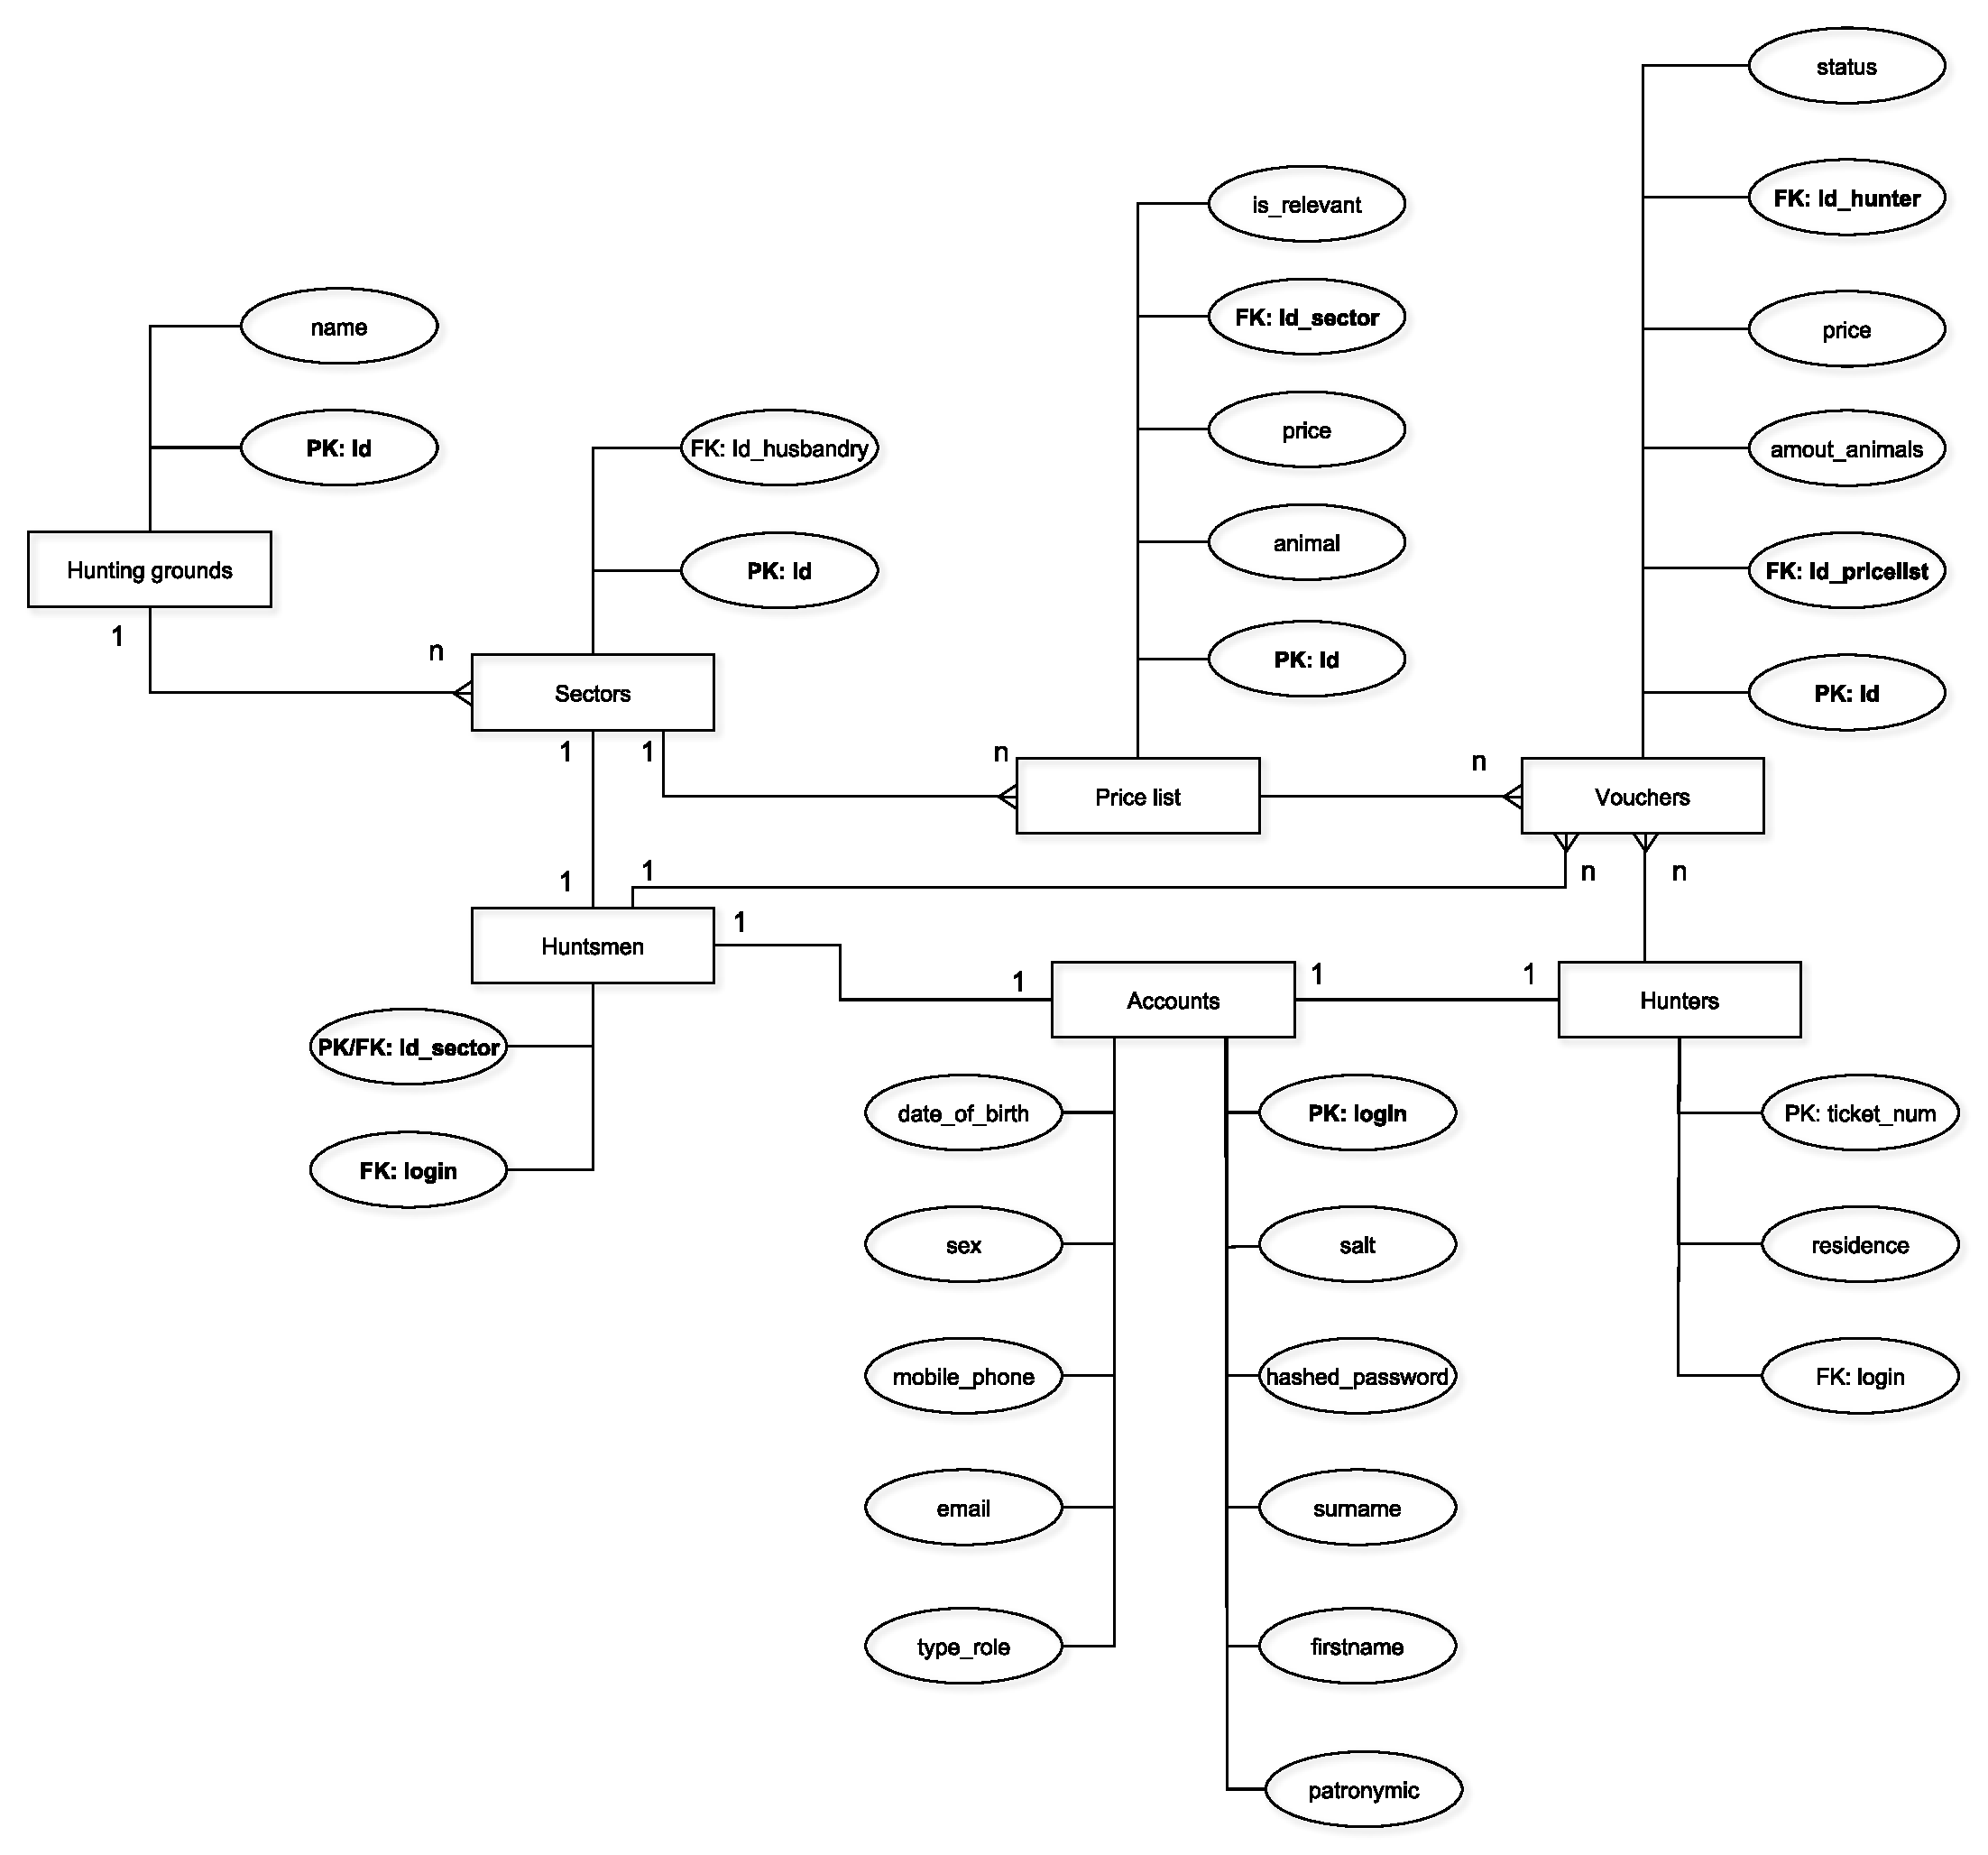
\includegraphics[scale=0.47]{schemes/ERclassic.pdf}}
			\caption{ER-диаграмма сущностей}
			\label{fig5:image}
		\end{center}
	\end{figure}

	\subsubsection{Проектирование базы данных}

	База данных должна содержать таблицы, поля и назначение которых описаны в таблицах 
	\ref{hgtable}-\ref{vouchers_table}.
	
	\begin{table}[h] 
		\begin{center}
			\caption{HuntingGrounds (таблица хозяйств)}
			\label{hgtable}
			\begin{tabular}{| p{3cm} | p{3cm} | p{8cm} |}
				\hline
				\textbf{Атрибут} 	& \textbf{Тип} & \textbf{Значение} \\
				\hline
				Id 					& Целое число &	Идентификатор, PK \\ 
				\hline
				GroundName 			& Строка &	Название \\ 
				\hline
			\end{tabular}
		\end{center}
	\end{table}

	\begin{table}[h] 
		\begin{center}
			\caption{Sectors (таблица секторов)}
			\label{sec_table}
			\begin{tabular}{| p{3cm} | p{3cm} | p{8cm} |}
				\hline
				\textbf{Атрибут} 	& \textbf{Тип} & \textbf{Значение} \\
				\hline
				Id 					& Целое число &	Идентификатор, PK \\ 
				\hline
				IdHusbandry 		& Целое число &	Идентификатор хозяйства, в состав которого входит сектор, FK \\
				\hline
			\end{tabular}
		\end{center}
	\end{table}

	\begin{table}[pt!]
		\begin{center}
			\caption{Accounts (таблица аккаунтов)}
			\label{acc_table}
			\begin{tabular}{| p{3cm} | p{3cm} | p{8cm} |}
				\hline
				\textbf{Атрибут} 	& \textbf{Тип} & \textbf{Значение} \\
				\hline
				Login 				& Строка &	Логин, PK \\ 
				\hline
				Salt 				& Строка &	Соль  \\ 
				\hline
				HashedPassword 		& Строка &	Хэшированный пароль \\ 
				\hline
				Surname 			& Строка &	Фамилия \\ 
				\hline
				Firstname 			& Строка &	Имя \\ 
				\hline
				Patronymic 			& Строка &	Отчество \\ 
				\hline
				DateOfBirth 		& Дата &	Дата рождения \\ 
				\hline
				Sex 				& Символ &	Пол \\ 
				\hline
				MobilePhone 		& Строка &	Мобильный телефон \\ 
				\hline
				Email 				& Строка &	Электронная почта \\ 
				\hline
				TypeRole 			& Строка &	Роль \\ 
				\hline
			\end{tabular}
		\end{center}
	\end{table}

	Для обеспечения безопасности используется хэширование паролей, и в базе данных в таблице \ref{acc_table} хранится только соль и хэшированный пароль.\\

	\begin{table}[pt!] 
		\begin{center}
			\caption{Huntsmen (таблица егерей)}
			\label{huntsmen_table}
			\begin{tabular}{| p{3cm} | p{3cm} | p{8cm} |}
				\hline
				\textbf{Атрибут} 	& \textbf{Тип} & \textbf{Значение} \\
				\hline
				Id 					& Целое число &	Идентификатор сектора, за которым закреплён егерь, PK, FK \\
				\hline
				Login	 			& Строка &	Логин, FK \\ 
				\hline
			\end{tabular}
		\end{center}
	\end{table}

	\begin{table}[pt!] 
		\begin{center}
			\caption{Hunters (таблица охотников)}
			\label{hunters_table}
			\begin{tabular}{| p{3cm} | p{3cm} | p{8cm} |}
				\hline
				\textbf{Атрибут} 	& \textbf{Тип} & \textbf{Значение} \\
				\hline
				TicketNum 			& Строка &	Номер охотничьего билета, PK\\
				\hline
				Residence			& Строка & 	Адрес прописки \\
				\hline
				Login	 			& Строка &	Логин, FK \\ 
				\hline
			\end{tabular}
		\end{center}
	\end{table}

	\begin{table}[pt!]
		\begin{center}
			\caption{PriceList (таблица цен на путёвки)}
			\label{price_table}
			\begin{tabular}{| p{3cm} | p{3cm} | p{8cm} |}
				\hline
				\textbf{Атрибут} 	& \textbf{Тип} & \textbf{Значение} \\
				\hline
				Id 					& Целое число &	Идентификатор, PK\\
				\hline
				Animal				& Строка & 	Название животного \\
				\hline
				Price	 			& Вещественное число &	Цена \\ 
				\hline
				IsRelevant	 		& Логический &	Флаг актуальности \\ 
				\hline
				IdSector	 		& Целое число &	Идентификатор сектора, за которым закреплена позиция, FK \\
				\hline
			\end{tabular}
		\end{center}
	\end{table}

	\begin{table}[pt!] 
		\begin{center}
			\caption{Vouchers (таблица путёвок)}
			\label{vouchers_table}
			\begin{tabular}{| p{3cm} | p{3cm} | p{8cm} |}
				\hline
				\textbf{Атрибут} 	& \textbf{Тип} & \textbf{Значение} \\
				\hline
				Id 					& Целое число &	Идентификатор, PK\\
				\hline
				AmountAnimals		& Целое число & 	Количество животных \\
				\hline
				Price	 			& Вещественное число &	Цена \\ 
				\hline
				IdHunter	 		& Строка &	Идентификатор владельца-охотника, FK \\ 
				\hline
				IdPricelist	 		& Целое число &	Идентификатор позиции из перечня цен, FK \\
				\hline
				Status				& Логический & 	Статус (ждёт решения/одобрено) \\
				\hline
			\end{tabular}
		\end{center}
	\end{table}

	\subsection{Нормальная форма модели}
	Распространённый подход к проектированию базы данных - метод нормализации, в результате получается одна из нормальных форм:
	\begin{itemize}
		\item первая нормальная форма (1НФ или 1NF);
		\item вторая нормальная форма (2НФ или 2NF);
		\item третья нормальная форма (3НФ или 3NF);
		\item и т.д.
	\end{itemize}

	В виду особенностей поставленной задачи, третья нормальная форма является наиболее предпочтительной.\\
	
	В разработанной модели переменные отношения находится в первой нормальной форме, поскольку все атрибуты являются простыми. В реляционной модели отношение всегда находится в 1НФ.\\
	
	Также все неключевые атрибуты полностью зависят от первичного ключа, что говорит о том, что отношение находится во 2НФ. \cite{NF} \\
	
	В силу того, что неключевые атрибуты не связаны отношениями между собой, можно сделать вывод о том, что транзитивных зависимостей нет, и переменная отношения находится в 3НФ. \\
	
	\subsection{Схемы триггеров}
	Триггеры автоматически выполняются при наступлении заданного события. Поэтому с их помощью можно успешно реализовывать некоторые действия. Для обеспечения целостности данных требуется реализовать следующие триггеры.
	\begin{itemize}
		\item Триггер, запрещающий удалять администратора, если в системе он остался единственным. Если его удалить, то часть функционала (такая как рассмотрение заявок на регистрацию пользователей, удаление аккаунтов и т.д.) перестанет быть доступной. Схема изображена на рисунке \ref{fig35:image}.
		
		\begin{figure}[h]
			\centering
			\begin{center}
				{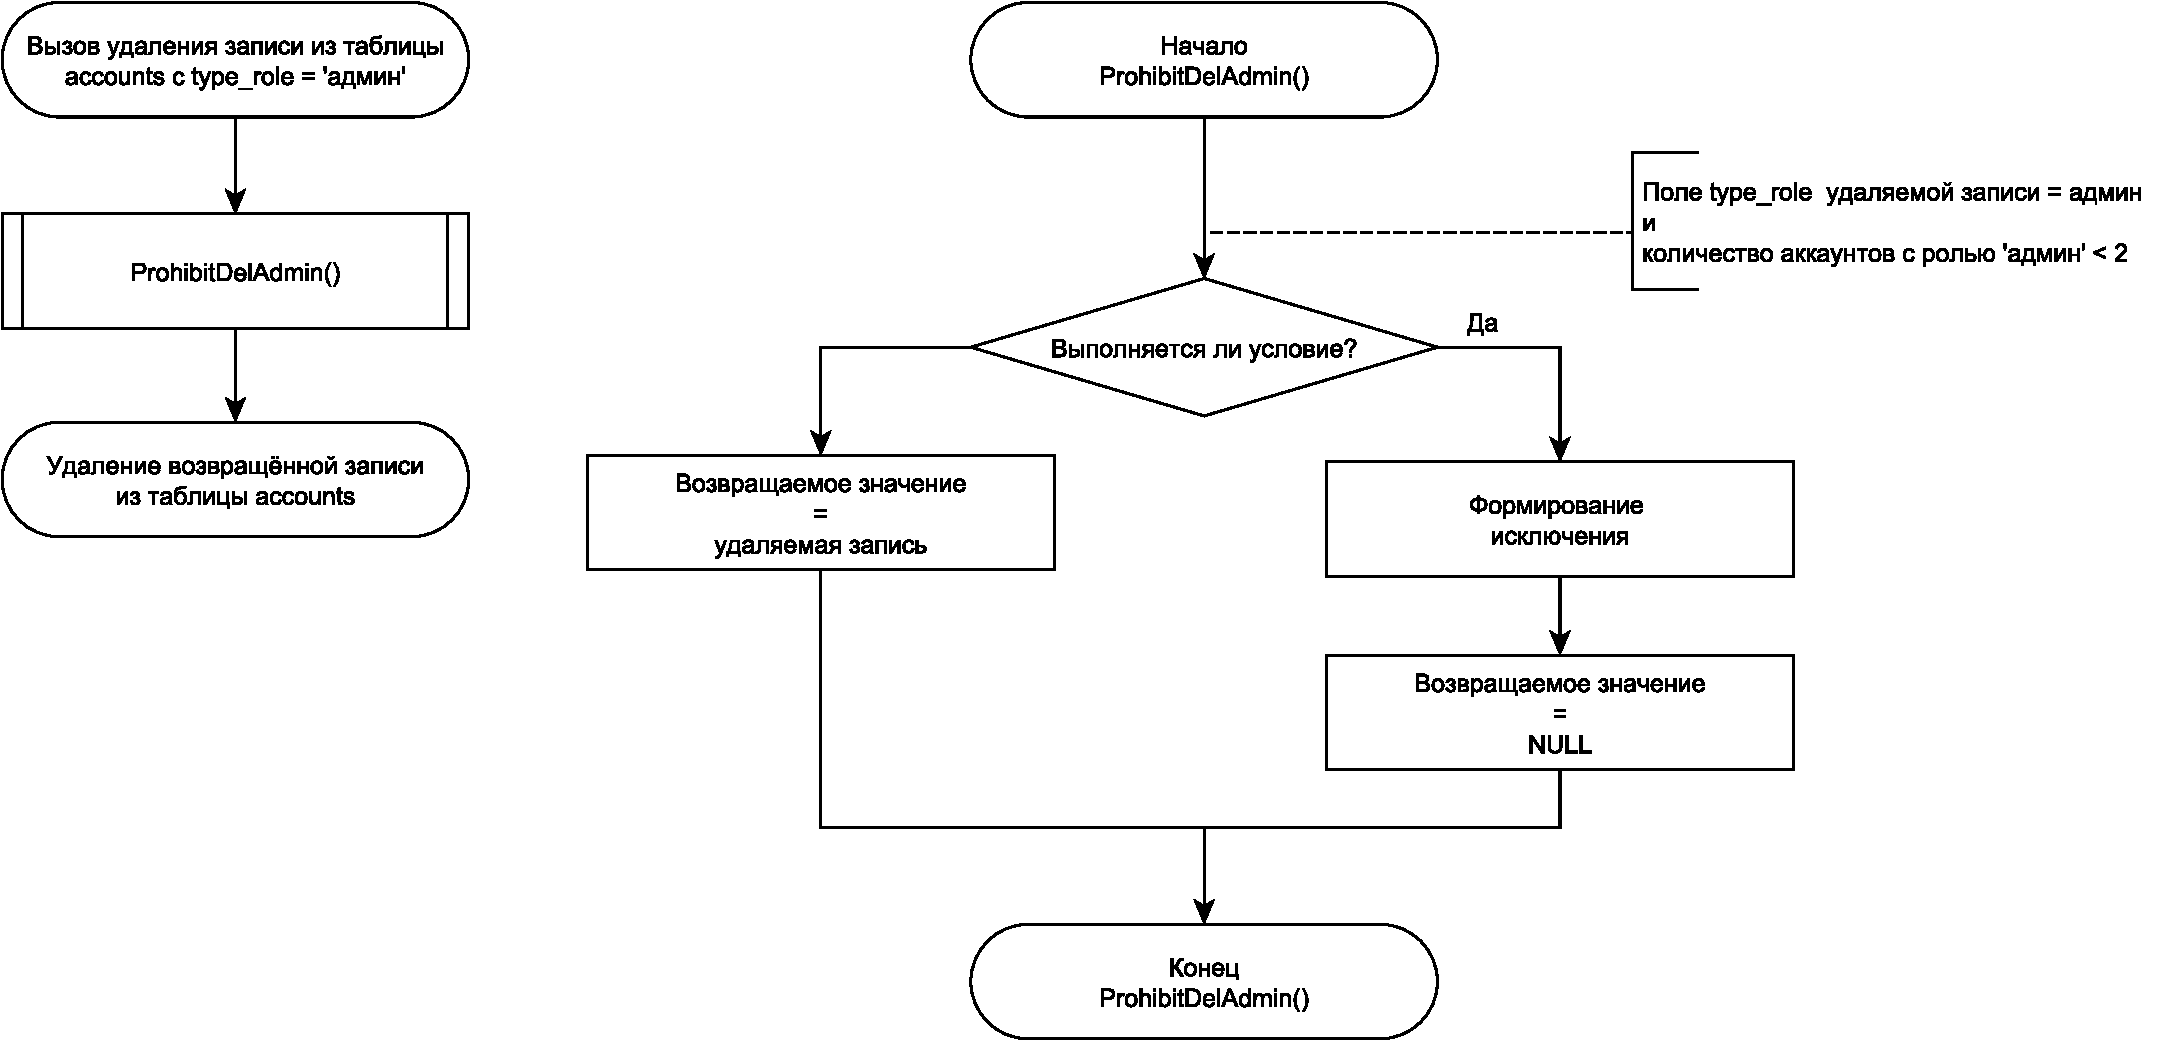
\includegraphics[scale=0.45]{schemes/triggeradmin.pdf}}
				\caption{Схема триггера, запрещающего удалять последнего администратора}
				\label{fig35:image}
			\end{center}
		\end{figure}
	
		\item Триггер на удаление связанных с охотником записей в других таблицах. Поскольку информация, касающаяся охотника хранится в нескольких таблицах, важно следить за корректным удалением данных во избежании ошибок. Схема такого триггера представлена на рисунке \ref{fig36:image}.
		
		\begin{figure}[h!]
			\centering
			\begin{center}
				{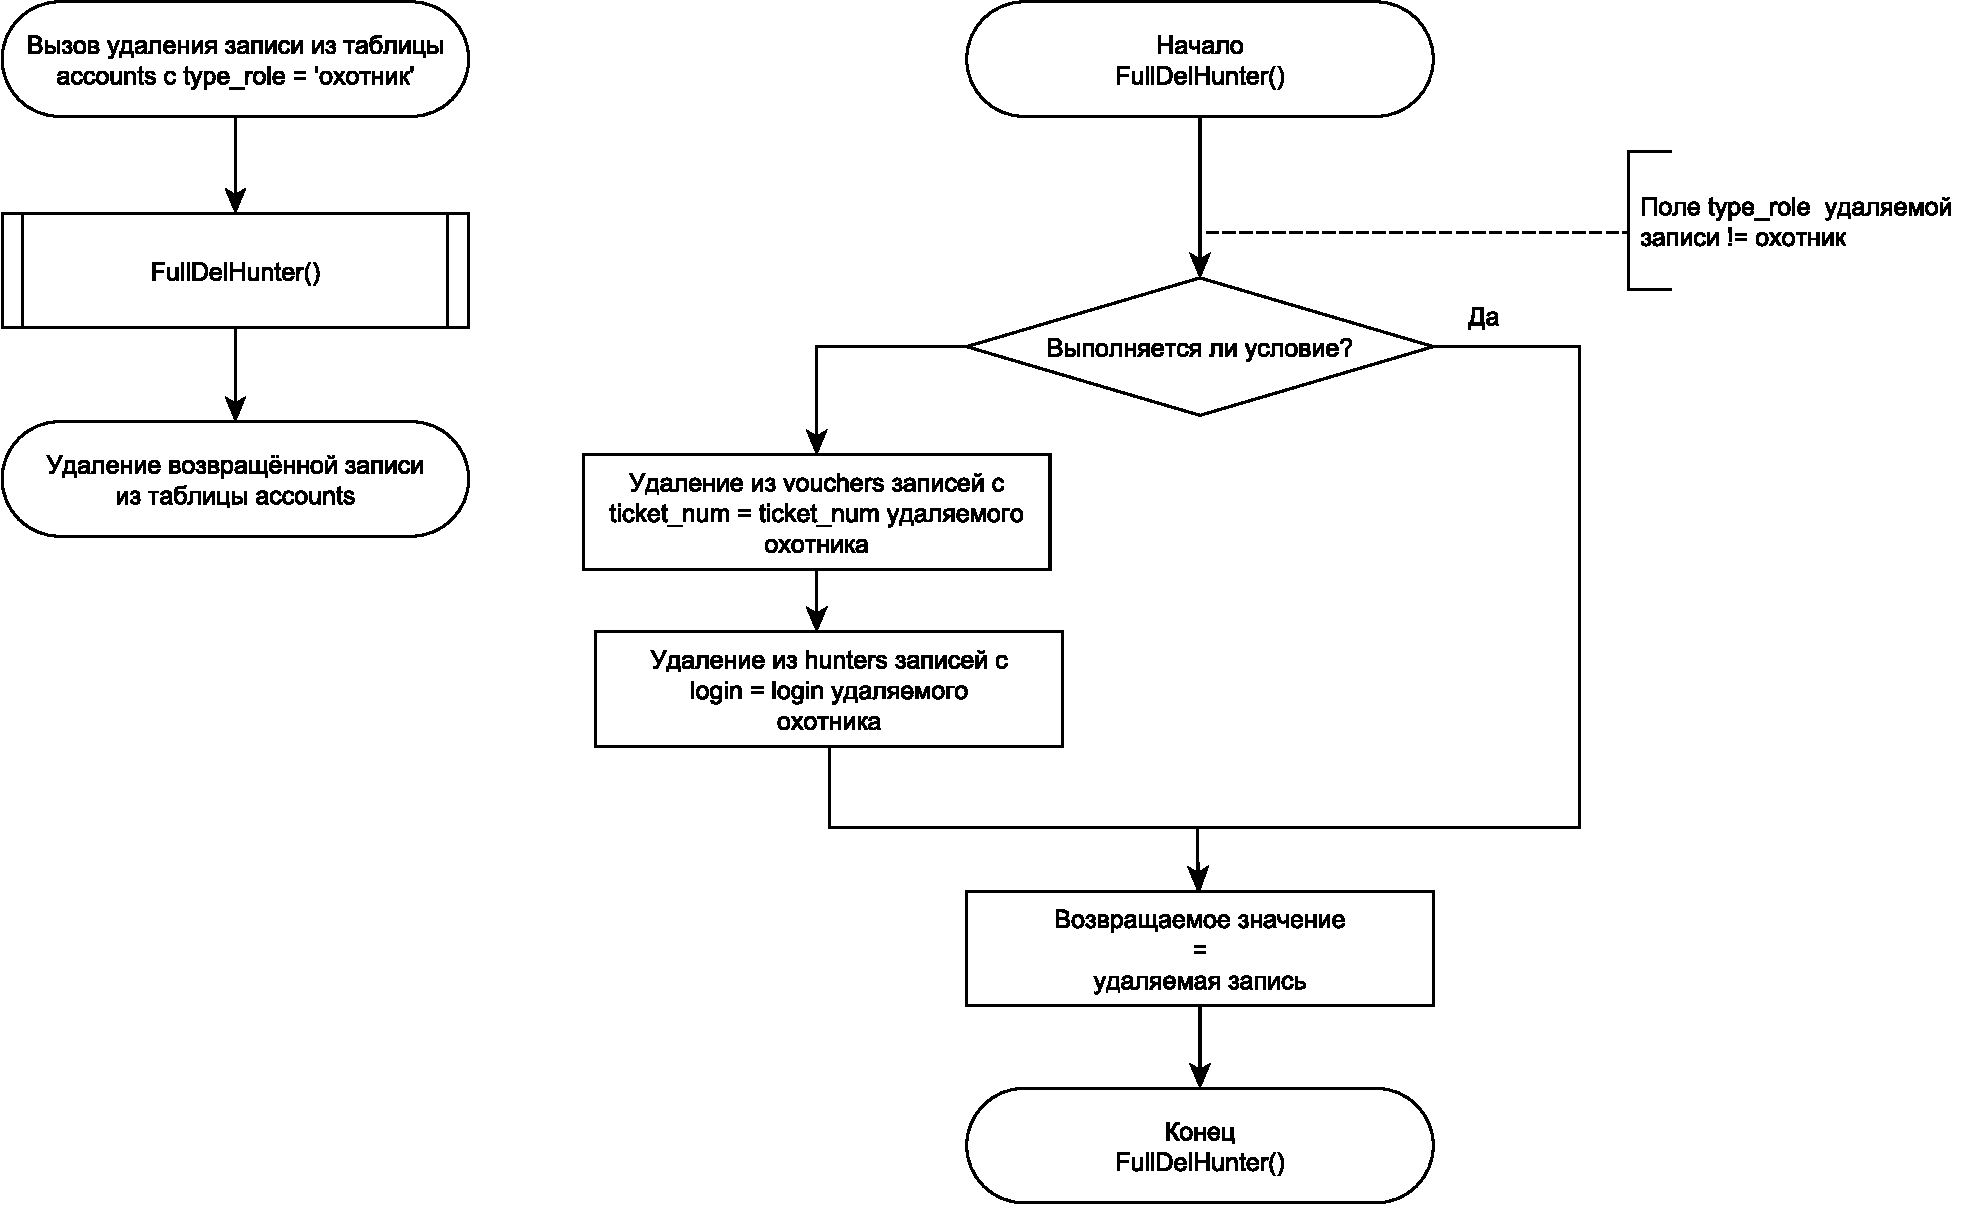
\includegraphics[scale=0.45]{schemes/trigger_delhunter.pdf}}
				\caption{Схема триггера на удаление связанных с охотником записей в других таблицах}
				\label{fig36:image}
			\end{center}
		\end{figure}
		\newpage
	
		\item Триггер на удаление связанных с егерем записей в других таблицах. Смысл такой же, как и у предыдущего триггера. Соответствующая схема изображена на рисунке \ref{fig37:image}.
		
		\begin{figure}[h!]
			\centering
			\begin{center}
				{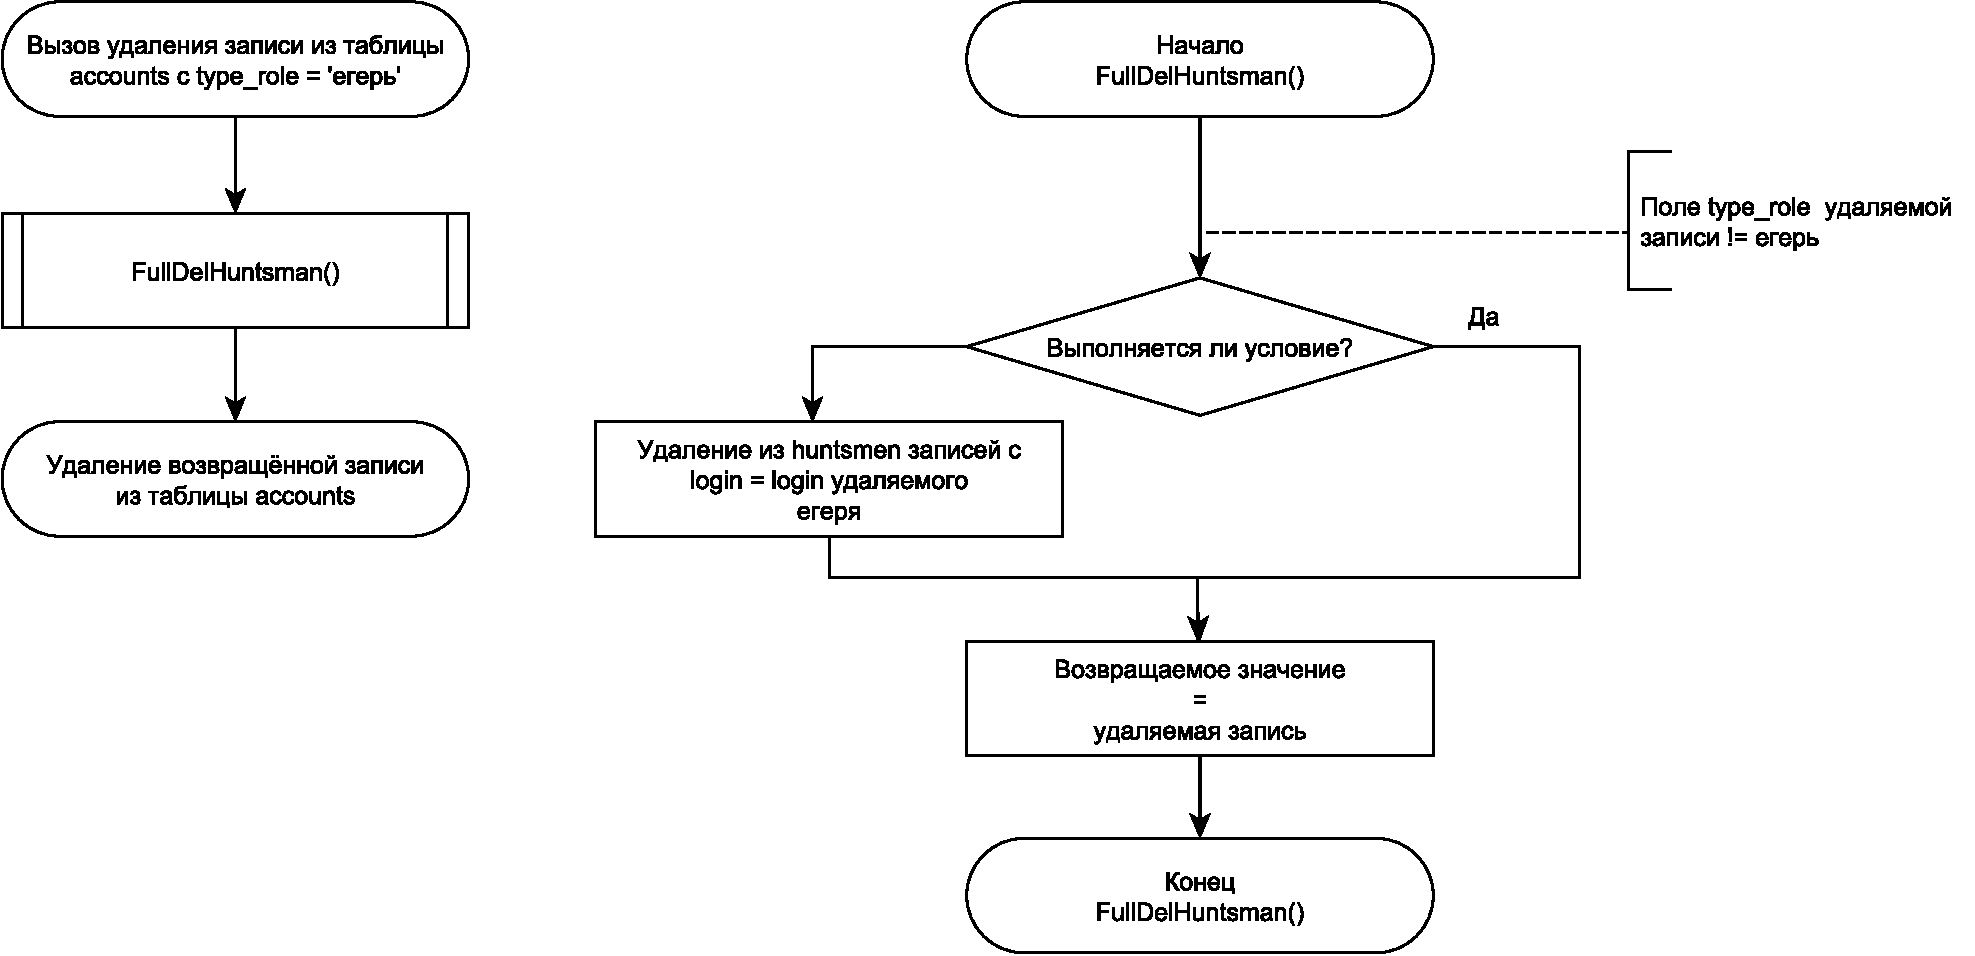
\includegraphics[scale=0.45]{schemes/trigger_delhuntsman.pdf}}
				\caption{Схема триггера на удаление связанных с егерем записей в других таблицах}
				\label{fig37:image}
			\end{center}
		\end{figure}
	
		\item При добавлении в базу данных нового егеря необходимо соблюдать условие, что за одним сектором может быть закреплён только один егерь, поэтому при выполнении данной операции важно учитывать это условие. Можно осуществлять подобную проверку с помощью триггера, схема которого представлена на рисунке \ref{fig38:image}.
		
		\begin{figure}[h!]
			\centering
			\begin{center}
				{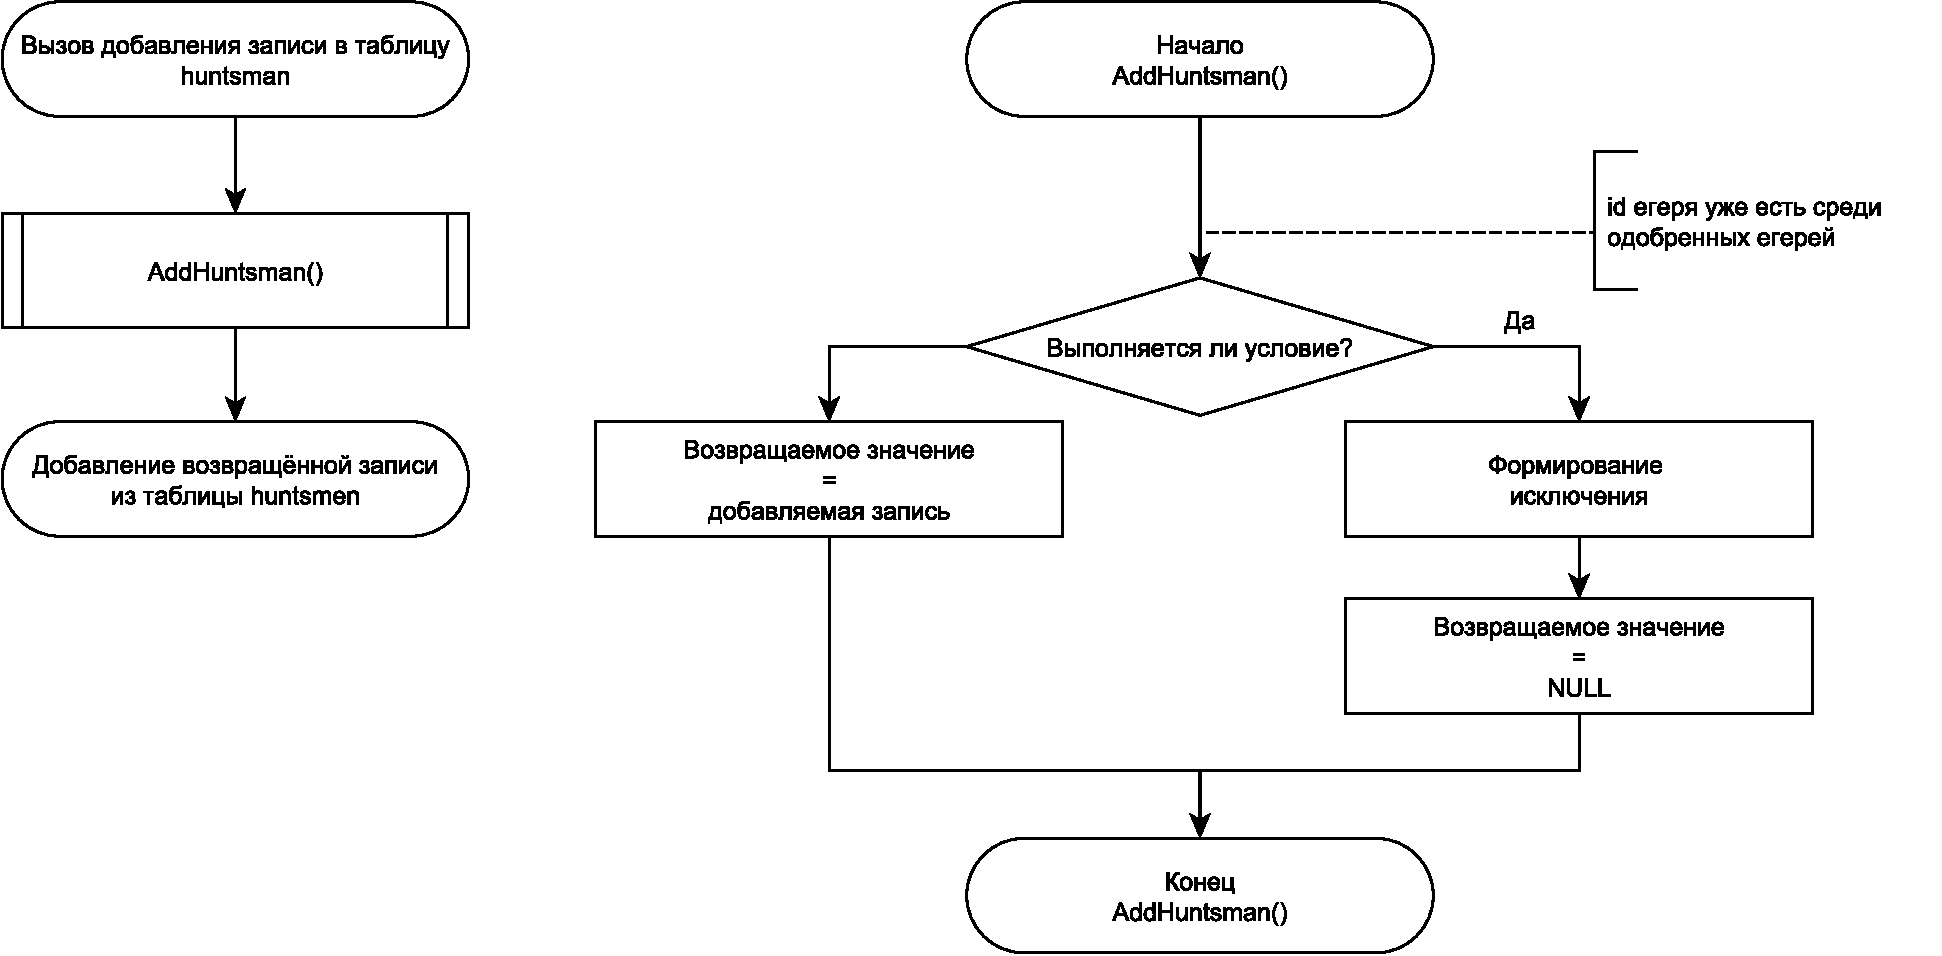
\includegraphics[scale=0.45]{schemes/trigger_addhuntsman.pdf}}
				\caption{Схема триггера, проверяющего единственность егеря в секторе}
				\label{fig38:image}
			\end{center}
		\end{figure}
		
		
	\end{itemize}

	\subsection{Архитектура приложения. Модель MVC}
	Этот шаблон проектирования предполагает разделение приложения на три отдельных компонента: Модель (Model), Представление (View) и Контроллер (Controller). Это позволяет производить модификации какого-либо компонента независимо от других. \cite{mvc} 
	
	\textbf{Model} - компонент бизнес-логики приложения, предоставляет данные и методы работы с ними.
	
	\textbf{View} - компонент, который отвечает за взаимодействие с пользователем, необходим для отображения данных, полученных в результате работы модели.
	
	\textbf{Controller} отвечает за обработку действий пользователя, перенаправляет данные от пользователя к модели и наоборот.\\
	
	\subsection*{Вывод}
	В разделе были представлены: Use-Case диаграммы для каждой из выделенных ролей (администратора, егеря и охотника), ER-диаграмма сущностей базы данных и триггеры, которые необходимо в дальнейшем реализовать. Также описана модель MVC, которая была выбрана для дальнейшей реализации. 




	
	